\documentclass[../main.tex]{subfiles}


\begin{document}

\chapter{Design}
\label{chap:design}

This chapter describes and justifies the protocol designed in the context of this thesis.
The main purpose of the protocol is to share encrypted logs with multiple parties.
In the previous \cref{chap:overview}, possible encryption strategies were introduced and evaluated based on the identified system requirements (see \cref{chap:requirements}).
Hybrid encryption was identified as the most promising encryption technique.
The evaluation of the protocol in terms of functionality, security, and performance can be found in \cref{chap:evaluation}.

A high-level overview of the designed protocol can be found in \cref{sec:overview}.
Different design considerations for the protocol are discussed in \cref{sec:protocol-considerations}.
The imposed algorithms to create, encrypt, and decrypt logs are explained in the subsequent sections. 

\section{Protocol overview}
\label{sec:overview}

The implemented protocol extends the current toolchain because it supports encrypted logs.
Additionally, access to encrypted logs can be shared and revoked by the data owner.

The protocol relies on an established PKI.
Each user requires two key pairs.
The first key pair is dedicated to encrypting data.
Its public key is called the encryption key while its private key is called the decryption key.
The second key pair is intended to sign data.
Its public key is called the verification key while its private key is called the signing key.
Public keys are represented by PEM-encoded certificates signed by a trusted CA.
Private keys are represented by a PEM-encoded private keys.
This separation of keys is considered to be the best practice in modern key management~\cite[33]{Barker2006}.
Each user must have exclusive access to its private keys.
The public keys of all users are expected to be publicly available in the system.
The protocol further assumes that a participating user has access to its key material, e.g. via hardware token.

The protocol relies on three fundamental cryptographic operations:
Signing, encrypting, and decrypting logs.
They are used to construct the full functionality of the demanded protocol.
They enable the exchange of end-to-end encrypted logs.
Moreover, they can be used to share and revoke access to logs.
The following description delivers a high-level overview of the functionality of the protocol.
This is additionally visualized in \cref{fig:protocol-overview}.

Whenever a monitor component observes a data access, it must create a log.
A log must always be a signed data structure.
Thus, the protocol requires the monitor to perform two tasks.
First, the raw log data needs to be cryptographically signed by the monitor.
Second, the log needs to be encrypted for the data owner.
The encrypted log is finally sent to the \emph{Safekeeper}.
This allows the data owner to request and decrypt the log.
The decryption process also involves validity checks of the received data.
This ensures that the protocol was applied correctly.

The data owner can share or revoke access to a log for other users.
Therefore, the data owner needs to download and decrypt the log from the server.
To share or revoke access to the log, the data owner applies the encryption algorithm with a set of desired users.
The access can be shared by adding additional users during encryption.
The access can be revoked by omitting users during encryption.
It is crucial to the protocol that the data owner always specifies itself within the set of authorized users.
Otherwise, the data owner cannot decrypt the log anymore.
Finally, the user uploads the log to the server.
Authorized users can download and decrypt the corresponding log.
Again, validity checks of the received data ensure that the defined security requirements are respected.

Note that the encryption algorithm can be applied by the monitor and the owner of the log.
Although only data owners are allowed to share and revoke access to logs, the log must be initially made available for the data owner.
This can be done by encrypting the log for the data owner:
Whenever a monitor created and signed a new log, it applies the encryption algorithm.
The only recipient for a new log must be the data owner.
To ensure that the monitor does not specify other unintended users, validation checks during decryption are mandatory.

\begin{figure}[h!]
    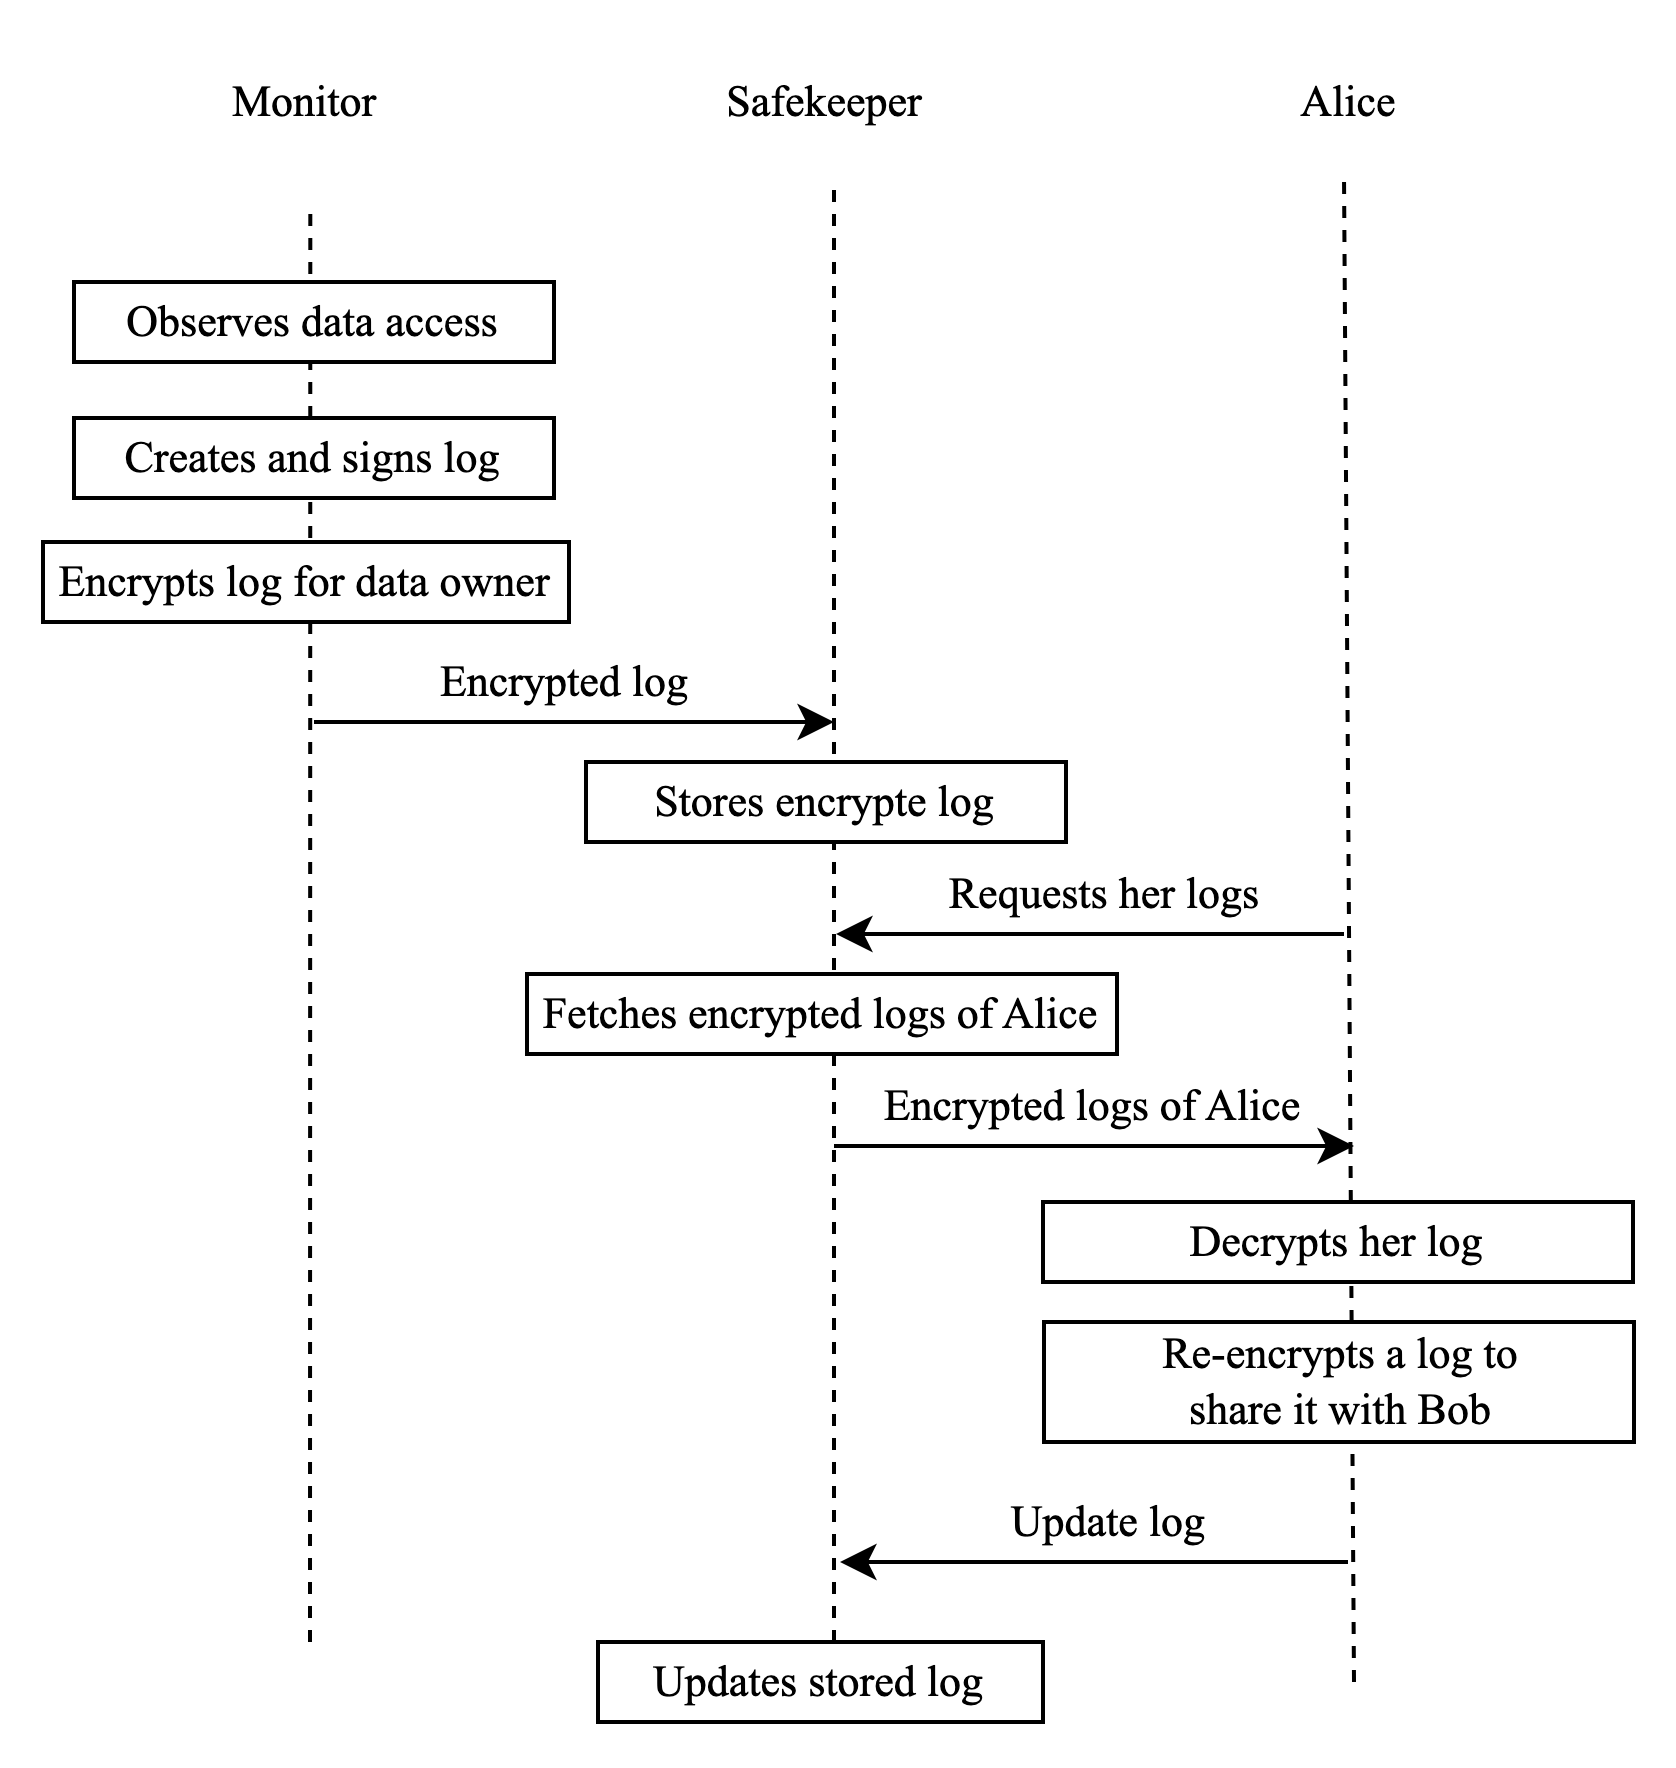
\includegraphics[width=12.7cm]{../img/05/overview.png}
    \centering
    \caption[Protocol overview]{
        The performed tasks and data flows when creating, and sharing logs in the toolchain.
        The monitor creates a log and encrypts it for Alice.
        Alice downloads and decrypts the log.
        Alice decides to share the log with Bob.
        Therefore, Alice re-encrypts the log and updates it in the \emph{Safekeeper} component.
        Revoking Bob's access requires Alice to re-encrypt the log while omitting Bob from the set of recipients.
    }
    \label{fig:protocol-overview}
\end{figure}

\section{General considerations}
\label{sec:protocol-considerations}
In this section, general design considerations of the protocol design are discussed.
\cref{sec:sign-and-encrypt} evaluates the secure combination of encryption and authentication mechanisms.
To design a practical and efficient protocol, intermediate servers are dependent on metadata.
This is elaborated in \cref{sec:metadata}.
Finally, \cref{sec:jose-protocol} illustrates how the JOSE standard can be utilized to practically implement the protocol.

\subsection{Secure application of encryption and authentication}
\label{sec:sign-and-encrypt}
The protocol allows data owners to share encrypted logs with a set of recipients.
The recipients must verify the authenticity of the encrypted data because only the owner or the monitor of a log are allowed to encrypt it.
Thus, the creator of an encrypted log is required to digitally sign the sent data.
This arises the question of whether encrypted data should be signed (\emph{encrypt-then-sign}) or whether signed data should be encrypted (\emph{sign-then-encrypt}).
In general, the \emph{encrypt-then-sign} approach is considered less secure because a malicious entity could simply stripe the signature and sign the ciphertext using its secret key~\cite{Davis2001}.
This might lead to unintended flaws in the resulting protocol~\cite{JWT2015}.

The naive \emph{sign-then-encrypt} approach, however, suffers from surreptitious forwarding in certain scenarios~\cite{Davis2001}.
The use case of this protocol is affected by the flaw.
Consider a log that is signed by the data owner.
This signed log is then encrypted for a set of users including a malicious user.
Nothing prevents the malicious user from re-encrypting the received log for any other user in the system.
It could finally forward the re-encrypted data to its target.
The problem arises because the target cannot verify if the data owner has intended to share the log with him or her.
They only know that the log was signed by the data owner.
This flaw can be mitigated by explicitly signing the intended recipients.
This allows a recipient to ensure that the data was intentionally encrypted for him by the claimed creator.~\cite{Davis2001}

For the protocol designed in the context of this thesis, those considerations have two implications.
First, a log must be signed by the creator whenever it is shared.
The creator must additionally sign the set of intended recipients.
Note that the log itself is also a signed data structure.
The log must always be signed by the monitor specified within the log to avoid the forgery of logs.
This ensures the security requirement~S3.
The signature of the creator ensures that unauthorized sharing operations can be detected.
This fulfills the security requirement~S2.
This construction nests singed data structures into each other.
Details can be found in \cref{sec:encrypting}.
Second, the signed data must be encrypted for the specified recipients.
This produces a ciphertext that can only be decrypted by those recipients, which ensures the security requirement~S1.

\subsection{Metadata}
\label{sec:metadata}
The exchanged logs are always encrypted.
This affects the performance of the toolchain.
From the perspective of intermediate servers, an encrypted log does not provide any meaningful information.
Specifically, they do not know which users have access to a log.
Hence, the server cannot associate a log with the authorized users.
This introduces two practical problems.

The first problem occurs when Alice tries to request logs concerning her.
If the server cannot associate logs with users, it must reply with all logs stored in the system.
As a consequence, Alice receives many logs that she cannot decrypt.
Since the raw cipher does not tell her which logs are intended for her, Alice must try to decrypt all logs to find the logs encrypted under her public key.
This is very inefficient and requires a lot of computational power.
To avoid this, the set of recipients can be attached as metadata to the encrypted log.

The second problem occurs when Alice tries to share access to her log.
Consider Alice to be a data owner.
Alice wants to share her log with Bob.
Before the sharing process starts, the encrypted log is stored on the server.
Alice re-encrypts the log under the public key of Bob.
She authenticates against the server and tries to update the stored log.
The server, however, does not know if Alice is the legitimate owner of the stored log because it cannot associate users with a given log.
Thus, the server does not allow Alice to update her log.
To avoid this, the server must know the identity of the data owner for all logs.
This can be realized by attaching the identity of the owner as metadata to the encrypted log.

To mitigate these limitations, the set of receivers and the identity of the data owner must be accessible without decryption.
This information can be interpreted as routing information and must be attached as metadata to the encrypted logs.
It allows the server to filter logs concerning a particular user.
Moreover, the server can allow data owners to modify their encrypted logs.
This practically enables them to share and revoke access to logs.
The construction implies, however, that the data sent over the insecure network contains the set of recipients twice.
Once within the metadata and once within the encrypted data.

\subsection{Realization via JOSE}
\label{sec:jose-protocol}

A log within the current \emph{transparency toolchain} is represented by a JSON object.
This motivates the usage of the JOSE standard~\cite{Barnes2014}.
Details about it can be found in \cref{sec:jose}.
The JOSE standard can be used to cryptographically sign~(JWS) and encrypt~(JWE) JSON data.
It defines multiple algorithms that can be used.
Specifically, JWE tokens can be computed using hybrid encryption.
Since JWS and JWE tokens can also be nested into each other, JOSE can be used to realize the desired protocol by the following means:
\begin{itemize}
    \item 
    A log is a JWS token signed by the monitor.
    It is referred to as the inner JWS token because it is nested into another JWS token.
    \item 
    To encrypt a log, the creator computes a JWS token, which contains the log as a nested token.
    The token additionally contains the set of intended recipients and the identity of the owner.
    This outer JWS token is called a \emph{shared log} in the context of this protocol.
    See \cref{fig:nested-jws} for a visualization of the nested tokens.
    \item
    The \emph{shared log} is finally encrypted to obtain a JWE token.
    This token also contains the unencrypted metadata within its protected header.
    The metadata, however, is still integrity protected.
\end{itemize}


\begin{figure}[h!]
    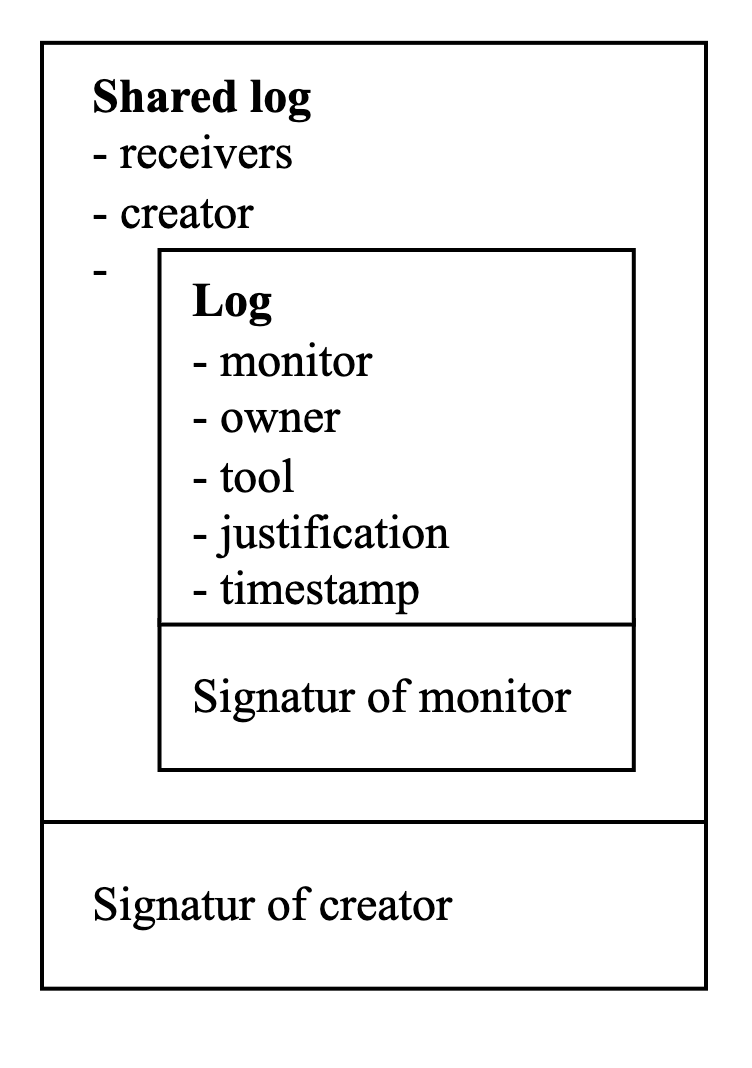
\includegraphics[width=5.5cm]{../img/05/nested_jws.png}
    \centering
    \caption[Nested JWS tokens]{A log is a JWS token signed by the monitor. A shared log is a JWS token that contains a nested log. It is signed by the entity encrypting the log.}
    \label{fig:nested-jws}
\end{figure}


\section{Creating logs}
\label{sec:signing}
A log is represented by a JWS token.
It contains the identity of the owner, the identity of the monitor, and further information that is relevant to identify the data access (see \cref{fig:nested-jws}).
To avoid malicious data owners manipulating or creating new logs, each log needs to be signed by the monitor specified within the log.
To create a JWS token, the monitor requires access to its private signing key.
A log is signed with the algorithm ES256, which relies on ECDSA and SHA-256.
It is defined by the "JSON Web Algorithm" specification~\cite{JWA2015}.
The log is later used as input for the encryption algorithm.
This construction is intended to resolve security requirement S3 because it allows decrypting users to verify if the provided log was indeed created by the claimed monitor.
This resists the attack of a malicious data owner trying to forge logs.

\section{Encrypting logs}\label{sec:encrypting}

The encryption algorithm requires two input parameters: A log and the set of users who are allowed to access the log.
It can be performed either by a monitor or the data owner.
A monitor initially encrypts the log for the data owner.
The monitor must not include his own identity in the set of authorized users.
More specifically, the set of authorized users must only contain the data owner if a monitor initially encrypts a log.
The data owner of the log might decide to share or revoke access to a log for users later on.
This requires the re-encryption of the log.
The data owner must always include his own identity in the set of authorized users.
The encryption algorithm outputs a JWE token, which can be decrypted by the specified users.

Internally, the encryption algorithm creates another JWS token.
This token is signed with the private signing key of the user encrypting the log (i.e. the creator).
It is called a \emph{shared log} because it contains a nested log plus the set of recipients plus the identity of the creator (see \cref{fig:nested-jws}).
The latter allows a decrypting user to download the public key of the creator, which is used to verify the signature of the \emph{shared log}.
The set of recipients is included to mitigate surreptitious forwarding.
This construction is intended to resolve security requirement S2.
It allows to verify whether the data owner has intended to share the log with a respective receiver.
This resists surreptitious forwarding attacks~\cite{Davis2001}.

Once the  shared log is created, it is used to compute the final JWE token.
Details about JWE tokens can be found in \cref{sec:jwe}.
This computation follows the \emph{sign-then-encrypt} approach elaborated in \cref{sec:sign-and-encrypt}.
The final token is computed by passing the encoded shared log as plaintext into the JWE encryption algorithm.
The identities of recipients and the identity of the owner are additionally passed as metadata into the protected header of the JWE token.
The choice of used algorithms to encrypt the data implies hybrid encryption.
The plaintext is encrypted with the authenticated encryption algorithm \verb|A256GCM|.
This is a symmetric encryption algorithm based on 256-bit AES using the Galois/Counter-Mode~\cite{JWA2015}.
The used symmetric key must then be encrypted for each intended recipient.
This allows the distribution of the key to all recipients.
It is realized using the key-wrapping algorithm \verb|ECDH-ES+A256KW|.
The algorithm returns a cipher that can be decrypted by the receiver.
It must be executed once for each receiver.
The specification of \verb|ECDH-ES+A256KW| requires the following steps to encrypt the symmetric key $k$ for a single receiver~\cite[100]{Barker2017}.
This is also illustrated in \cref{fig:key_wrapping}.
\begin{figure}[ht]
    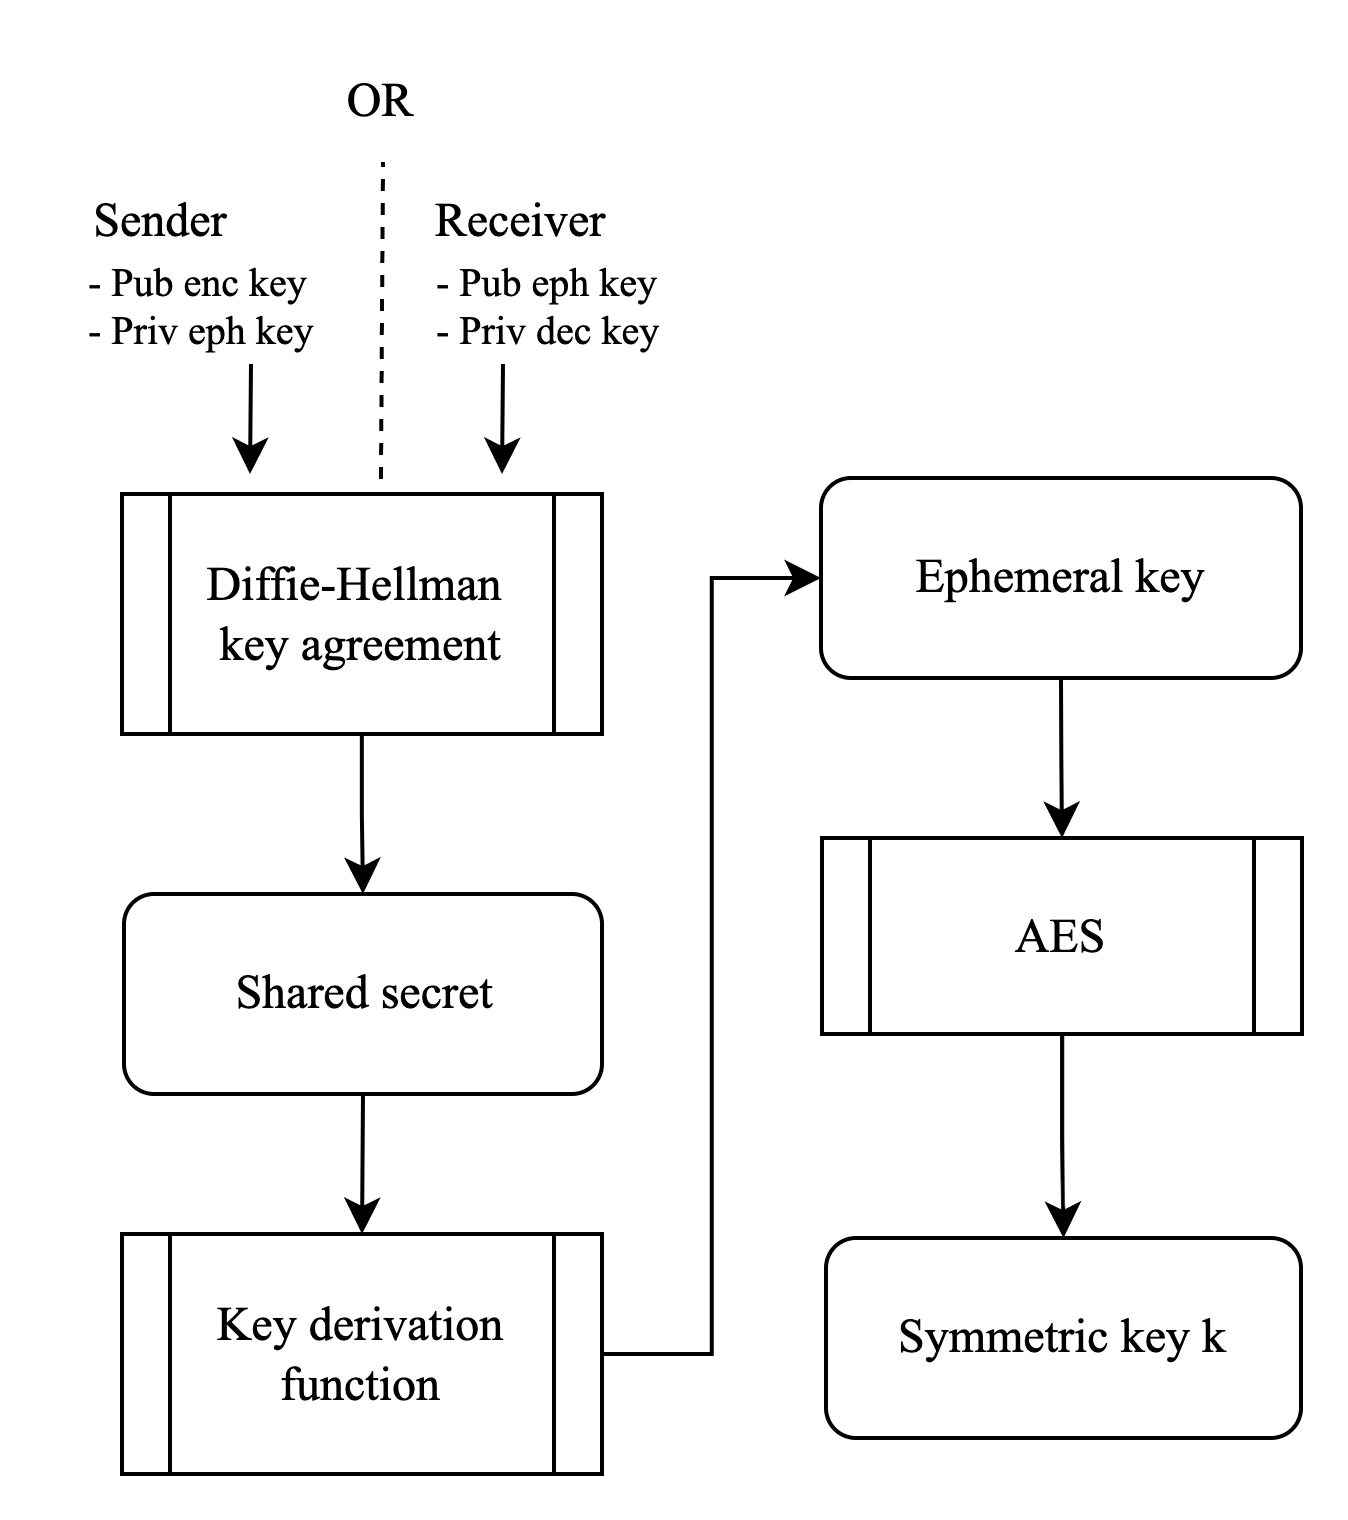
\includegraphics[scale=0.2]{../img/05/key_wrapping.png}
    \centering
    \caption[Key-wrapping ECDH-ES+A256KW]{
        Key-wrapping of the symmetric key k using ECDH-ES+A256KW.
        Based on the exchanged public keys the sender and receiver can both compute the same shared secret.
        The derived ephemeral key is finally used to encrypt/decrypt the symmetric encryption key k under AES.}
    \label{fig:key_wrapping}
\end{figure}

\begin{enumerate}
    \item 
    The sender must know the static public key of the receiver. 
    In our case, this is the public encryption key.
    The receiver must have exclusive access to its static private key.
    In our case, this is the private decryption key.
    \item 
    The sender creates a new ephemeral key pair. 
    This key pair must be used only once.
    \item 
    The sender sends the ephemeral public key to the receiver.
    In our case, the key is encoded into the JWE token.
    The ephemeral private key must be kept secret.
    \item 
    The sender knows the static public key of the receiver and the ephemeral private key of the sender.
    The receiver knows the ephemeral public key of the sender and the static private key of the receiver.
    Thus, the Diffie-Hellman key agreement protocol can be used to compute a shared secret between the sender and the receiver~\cite[438]{Eckert2018}.
    The computation of the shared secret requires either the ephemeral private key or the static private key.
    If both are kept secret, it is assumed to be computationally infeasible to compute the shared secret~\cite[438]{Eckert2018}.
    \item 
    The shared secret, which is the result of the Diffie-Hellman key agreement protocol, is used as input for a key derivation function.
    This function computes an ephemeral key between the sender and the receiver.
    \item 
    Finally, this ephemeral key is used as key to encrypt the symmetric key $k$ for the receiver.
    This encryption uses the symmetric scheme AES.
\end{enumerate}


The resulting JWE token contains the symmetrically encrypted log, the encrypted keys for all recipients, and the protected header.
It can only be decrypted by the specified recipients because they are the only users who can restore the symmetric encryption key.
This is intended to resolve security requirement S1 because it effectively end-to-end encrypts a log.
Only explicitly authorized users can decrypt the log.
The whole encryption process is depicted in detail in \cref{app:encryption}.

\section{Decrypting logs}\label{sec:decrypting}

The decryption algorithm takes a JWE token and a private decryption key as input.
To verify the JWS tokens encoded within the JWE token, this algorithm needs to be able to dynamically resolve the identities of users to their public keys.

First of all, the JWE token is parsed into its ciphertext, header, and encrypted keys.
The JWE decryption algorithm is then applied to the cipher.
This decrypts the ciphertext using the passed private decryption key.
First, it tries to decrypt any of the encrypted keys provided in the JWE token using \verb|ECDH-ES+A256KW|.
If this succeeds, the symmetric encryption key is accessible.
This allows the decryption of the symmetric ciphertext using \verb|A256GCM|.
This effectively restores the \emph{shared log} for the receiver.
No decryption is necessary to access the metadata because is stored in the protected header of the JWE.
If the decryption is successful, the decrypting user has access to the \emph{shared log} and the metadata.
Multiple validations are necessary to ensure that the protocol is used correctly.
If any of them fails, the decryption must be aborted with an error.
\begin{enumerate}
    \item 
    The signature of the obtained \emph{shared log} (outer JWS token) must be validated.
    To do so, the decrypting user needs to download the public key of the creator specified in the \emph{shared log}.
    If the verification of the signature succeeds, the decrypting user can be sure that the claimed creator indeed signed the \emph{shared log}.
    \item
    The signature of the nested log (inner JWS token) must be validated.
    Again, the public key of the specified monitor needs to be downloaded.
    The PKI must ensure that this public key belongs to a valid and trusted monitor component.
    If the verification of the signature succeeds, the decrypting user can be sure that the claimed monitor indeed signed the log.
    \item
    The metadata includes the set of recipients.
    The \emph{shared log} also includes this information.
    Only if both sets are equal, the token was not modified during transit.
    \item
    The user applying the decryption must be part of the set of recipients.
    If this is true, the user can ensure that the creator intended to share the log with him or her.
    \item
    The owner specified in the metadata must be equal to the owner specified in the log.
    Only if both are equal, the token was not modified during transit.
    \item
    The log specifies the owner and the monitor of the log.
    The \emph{shared log} specifies the creator of the encrypted message.
    The creator must be either the owner or the monitor of the log.
    
    If the creator is equal to the monitor of the log, the monitor encrypted the message for the data owner.
    In this case, the decrypting user must be the data owner.
    The set of recipients must only contain the identity of the data owner because the monitor is not allowed to encrypt the log for other users.

    On the other hand, the creator can be equal to the owner of the log.
    This implies that the owner shared the log with other users.
    In this case, the set of recipients can be arbitrary.
\end{enumerate}
If all those validations succeed, the received log can be trusted.
A visualization of the decryption process can be found in \cref{app:decryption}

\end{document}
